\section{Реализация и тестирование}
Предложенный алгоритм был реализован на платформе .NET как часть проекта YaccConstructor; основным языком разработки являлся F\#~\cite{FSharp}. Ранее в рамках проекта был реализован RNGLR-алгоритм и генератор управляющих таблиц анализа для него. Управляющие таблицы RNGLR-алгоритма переиспользуются, поэтому внесения изменений в генератор не потребовалось. Также были переиспользованы структуры данных для структурированного в виде графа стека GSS и компактного представления разбора SPPF. 

Алгоритм был протестирован на различных наборах тестов. Для каждого теста специфицировалась грамматика на языке YARD и в явном задавался граф конечного автомата, ребра которого были промаркированы лексемами эталонной грамматики. Полученный в результате работы алгоритма лес разбора печатался в файл и проверялся на корректность. Тесты можно разделить на две категории.
\begin{itemize}
  \item \emph{Регрессионные тесты} проверяющие, что предложенный алгоритм выдаёт те же результаты, что и RNGLR-алгоритм, на линейном входе (конечном автомате, принимающем единственную строку). В данный набор вошли все тесты, ранее использованные для тестирования работоспособности реализации RNGLR-алгоритма в проекте YaccConstructor. 
  \item \emph{Тесты на работоспособность}, проверяющие, что алгоритм строит корректное представление леса разбора всех корректных выражений из входного регулярного множества. Входные графы для данного набора тестов содержали как ветвления, так и циклы. Отдельно были рассмотрены случаи вложенных ветвлений и вложенных циклов. На всех тестах алгоритм генерировал корректный лес разбора, игнорируя некорректные относительно эталонной грамматики цепочки.
\end{itemize}


\subsection{Экспериментальная оценка алгоритма}\label{SyntTestsEvalDescr}

Алгоритм синтаксического анализа динамически формируемых выражений, описанный выше, был протестирован на нескольких сериях синтетических тестов, цель которых~--- убедиться в приемлемой производительности алгоритма на практически значимых входных данных. Анализ промышленного проекта по миграции базы данных с MS-SQL Server 2005 на Oraclе 11gR2 показал, что запросы часто формируются конкатенацией фрагментов, каждый из которых формируется с помощью ветвлений или циклов. Ниже приведена эталонная грамматика $G_t$, использованная в этих тестах.

$$
\begin{array}{crcl}
& start\_rule &::=& s \\
& s & ::= & s \mbox{\texttt{ PLUS }} \mbox{\texttt{n}}\\
& n & ::= & \mbox{\texttt{ONE | }} \mbox{\texttt{TWO | }} \mbox{\texttt{THREE | }} \mbox{\texttt{FOUR | }} \\
&   &     & \mbox{\texttt{FIVE | }} \mbox{\texttt{SIX | }} \mbox{\texttt{SEVEN}}
\end{array}
$$

Входные данные представляли собой конечные автоматы над алфавитом терминальных символов грамматики $G_t$, построенные с помощью конкатенации базовых блоков. Предполагается, что такие графы могут быть получены в результате построения регулярной аппроксимации по некоторой программе и выполнения её лексического анализа. В данном случае базовый блок --- это шаблонный конечный автомат, который используется для построения тестовых конечных автоматов. Каждая серия тестов характеризовалась тремя параметрами: 

\begin{itemize}
  \item $height$~--- количество ветвлений в базовом блоке;
  \item $length$~--- максимальное количество повторений базовых блоков;
  \item $isCycle$~--- наличие в базовом блоке циклов (если ложь, то используются базовые блоки, изображённые на рисунке~\ref{block}, если истина~--- то изображённые на рисунке~\ref{block_loop}).
\end{itemize}

\begin{figure}[h!]
 \centering
 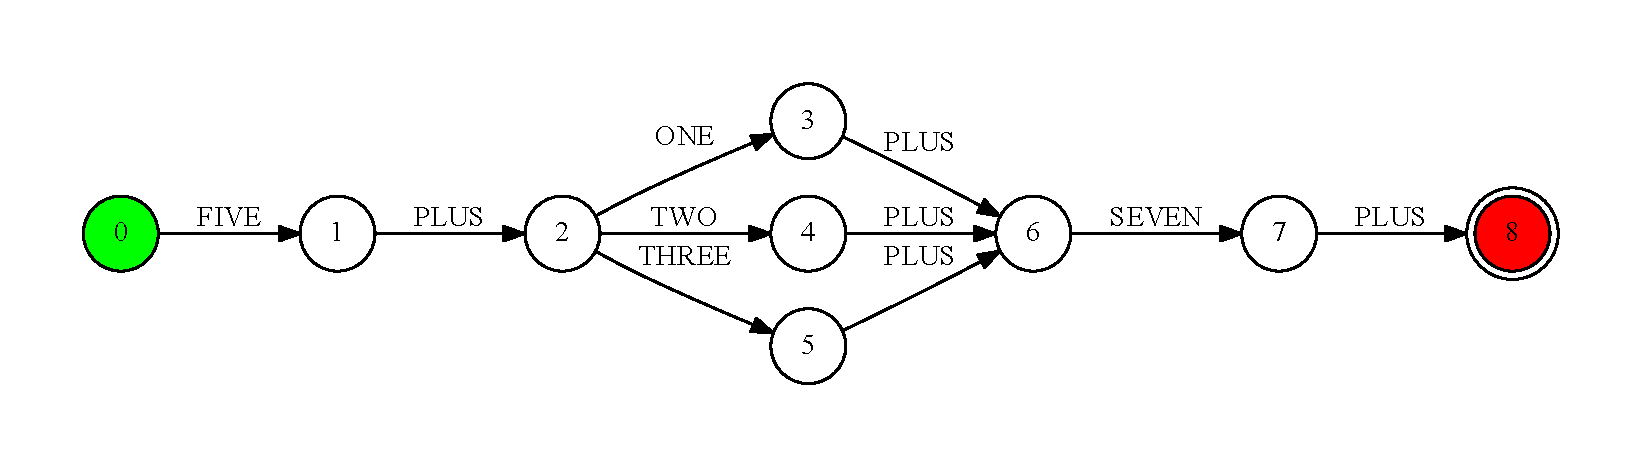
\includegraphics[width=15cm]{pics/block.pdf}
 \caption{Базовый блок без циклов при $height=3$}
 \label{block}
\end{figure}

\begin{figure}[h!]
 \centering
 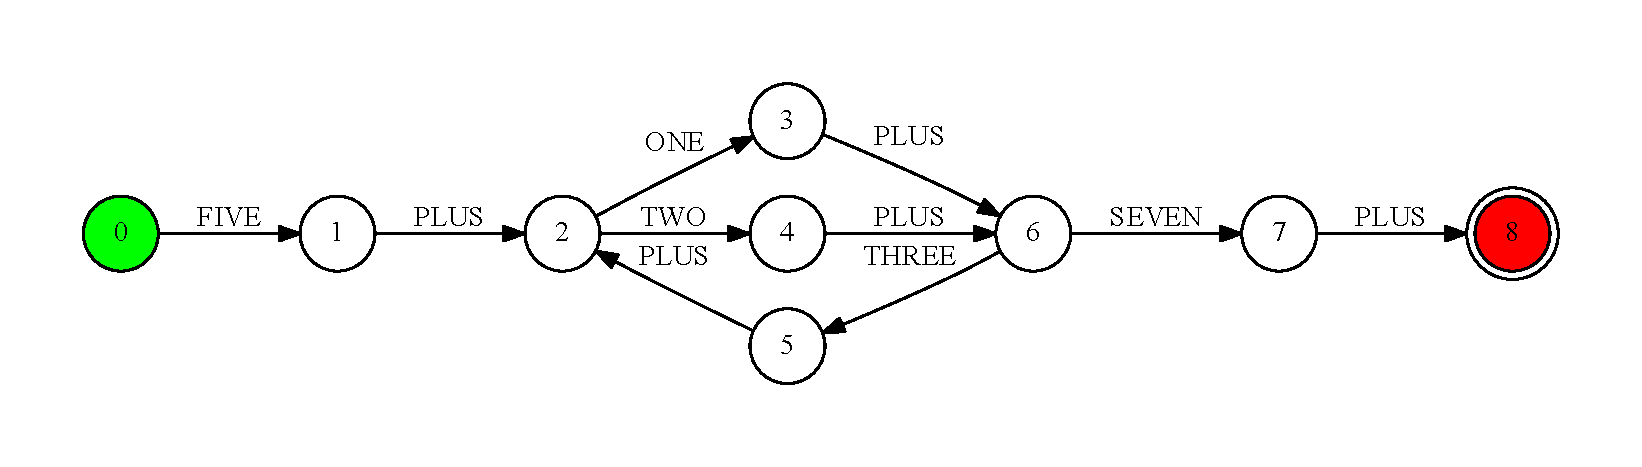
\includegraphics[width=15cm]{pics/block_loop.pdf}
 \caption{Базовый блок, содержащий цикл, при $height=3$}
 \label{block_loop}
\end{figure}

Замеры проводились на вычислительной станции со следующими характеристиками.
\begin{itemize}
\item Операционная система: Microsoft Windows 8.1 Pro
\item Тип системы: x64-based PC
\item Процессор: Intel(R) Core(TM) i7-4790 CPU @ 3.60GHz, 3601 Mhz, 4 Core(s), 8 Logical Processor(s)
\item Объём оперативной памяти: 16.0 GB
\end{itemize}

Чтобы выявить зависимость времени от размера входных данных, тесты проводились сериями. Каждая серия объединяет набор из $500$ тестов, каждый из которых содержит одинаковое количество ветвлений в базовом блоке. При этом количество повторений блока совпадает с порядковым номером теста, то есть $length=i$ для $i$-того теста. Для каждого теста измерялось время, затраченное на синтаксический анализ. Измерения проводились 10 раз, после чего усреднялись. График, представленный на рисунке~\ref{diffheights}, иллюстрирует зависимость времени, затрачиваемого на синтаксический анализ, от количества повторения базового блока и количества ветвлений в каждом из них. Можно заметить, что время, затрачиваемое на анализ, растёт линейно, в зависимости от размера входного графа. График на рисунке~\ref{CycleVsLinear} показывает, что наличие циклов в графе, при одинаковом значении параметра $height$, увеличивает продолжительность анализа, при этом зависимость времени от размера графа остаётся линейной.

\begin{figure}[h!]
 \centering
 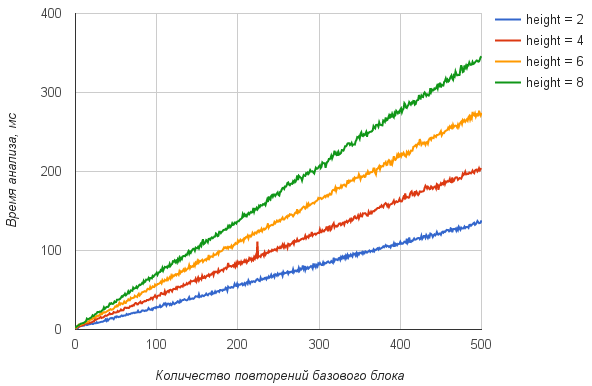
\includegraphics[width=15cm]{pics/diffheights.png}
 \caption{Зависимость времени работы алгоритма от размера входного графа при $isCycle=false$}
 \label{diffheights}
\end{figure}

\begin{figure}[h!]
 \centering
 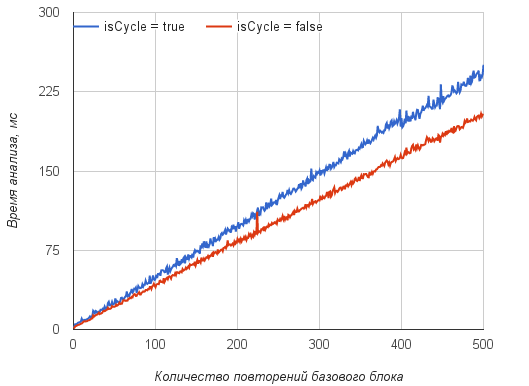
\includegraphics[width=15cm]{pics/heigh4.png}
 \caption{Зависимость времени работы алгоритма от размера входного графа и наличия в нем циклов при $height=4$}
 \label{CycleVsLinear}
\end{figure}


\subsection{Апробация в промышленном проекте по реинжинирингу}

Реализованный инструментарий был апробирован в рамках промышленного проекта по миграции базы данных с MS-SQL Server 2005 на Oraclе 11gR2, что позволило апробировать как предложенную архитектуру, так и протестировать некоторые части инструментария на реальных данных.

Обрабатываемая система состояла из 850 хранимых процедур и содержала около 2,6 миллионов строк кода. В ней присутствовало 2430 точек выполнения динамических запросов, из которых больше 75\% могли принимать более одного значения и при их формировании использовалось от 7 до 212 операторов. При этом среднее количество операторов для формирования запроса равнялось 40~\cite{Syrcose}.

Так как анализатор T-SQL был разработан ранее в рамках проекта, в котором происходило внедрение, то для создания анализатора встроенного SQL была использована готовая грамматика и по ней построен синтаксический анализатор. Построение регулярной аппроксимации и лексический анализ также были реализованы ранее в рамках основного проекта и были переиспользованы. Возможность использования компонент, созданных не в рамках YC.SEL.SDK, показало преимущества разделения шагов анализа.

Далее были реализованы функции вычисления метрик и вывода результата, после чего полученная функциональность была встроена в существующую цепочку обработки основного кода. В результате работы реализованных функций формировался отчёт, пример которого приведён в таблице~\ref{tbl:metrics}

Тесты проводились на вычислительном устройстве с параметрами, эквивалентными указанным в разделе~\ref{SyntTestsEvalDescr}. В ходе экспериментов измерялись следующие характеристики для каждой точки выполнения динамически формируемого запроса.

\begin{itemize}
  \item Время обработки t в миллисекундах. Проводилось 10 запусков, время анализа усреднялось. 
  \item Размер входного конечного автомата: количество состояний \#Q и количество переходов \#T.
  \item Размер построенного SPPF: количество вершин \#V и количество рёбер \#E.
  \item Результат анализа: $+$ --- завершился успешно, $-$ --- завершился с ошибкой, T --- завершён по таймауту.
\end{itemize} 


\begin{table} [htbp]
  \centering
  \parbox{14cm}{\caption{Распределение динамически формируемых SQL-запросов по времени обработки}\label{tbl:timing}}
  \begin{tabular}{| p{8cm} || p{3cm} | p{3cm}l |}
  \hline                               
  \hline
  Категория &\centering Количество запросов &\centering Время обработки (минуты) & \\
  \hline 
  Содержат корректные выражения                  &\centering  2188         &\centering  14& \\
  Не содержат ни одного корректного выражения    &\centering  240          &\centering  9& \\
  Обработка завершена по таймауту                &\centering  1            &\centering  4&  \\
  \hline
  \textbf{Всего}                                 &\centering \textbf{2430} &\centering \textbf{27} & \\
  \hline
  \hline
  \end{tabular}
\end{table}

Результаты измерений времени работы представлены в таблице~\ref{tbl:timing}. Алгоритм успешно завершил работу на 2188 входных графах, аппроксимирующих множества значений запросов. Ручная проверка входных графов, на которых алгоритм завершался с ошибкой, показала, что они действительно не содержали ни одного корректного в эталонном языке выражения. Причиной этого стала либо некорректная работа лексического анализатора, либо наличие в выражениях конструкций, не поддержанных в существующей грамматике. Так как лексический анализатор и грамматика были полностью заимствованы из оригинального проекта, то наличие этих ошибок не является недоработками алгоритма синтаксического анализа. Общее время синтаксического анализа составило 27 минут, из них 13 минут было затрачено на разбор графов, не содержащих ни одного корректного выражения. Из них 256 секунд --- обработка одного графа (5747 рёбер и 3897 вершин), прерванная по таймауту. Дальнейшие значения приводятся только для графов, которые удалось проанализировать. 604 из этих графов прождали ровно одно значение и анализировалось не более 1 миллисекунды. На разбор 1790 графов ушло не более 10 миллисекунд. На анализ двух графов было затрачено более 2 минут: 152,215 и 151,793 секунд соответственно. Первый граф содержал 2454 вершин и 54335 рёбер, второй~--- 2212 вершин и 106020 рёбер. Распределение входных графов по промежуткам времени, затраченных на анализ, приведено на графике на рисунке~\ref{distr}.

\begin{figure}[H]
  \centering
 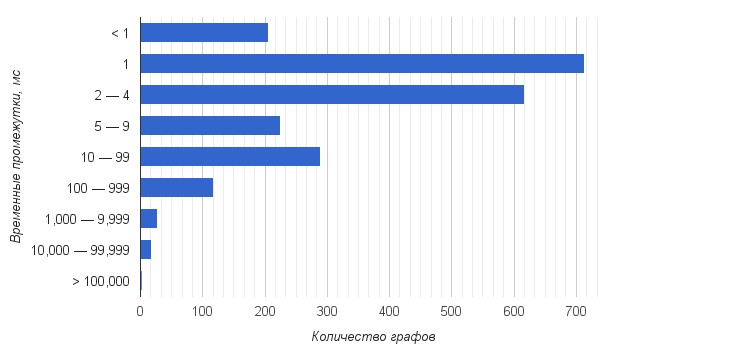
\includegraphics[width=0.95\textwidth]{pics/distr.png}
 \caption{Распределение запросов по времени анализа}
 \label{distr}
\end{figure}


\begin{table} [htbp]
  \centering
  \parbox{13cm}{\caption{Пример отчёта по результатам запуска синтаксического анализа на реальной системе}\label{tbl:metrics}}
  \begin{tabular}{| r | c | c | c | c | c | c |}
  \hline                               
  \hline
  \multirow{2}{*}{\textnumero} &\multirow{2}{*}{t(мс)} &\multirow{2}{*}{r} &\multicolumn{2}{c}{DFA} &\multicolumn{2}{|c|}{SPPF} \\
  \cline{4-7} 
                               &                   &                   & \#Q     & \#T          & \#V         &         \#E \\ 
  \hline 
1  &6      &$+$ &75  &76      &1074    &1075      \\
2  &73     &$+$ &104 &806   &18786   &26377   \\
3  &64     &$+$ &79  &750     &17237     &23954   \\
4    &15982  &$+$ &817 &32281 &920618    &1885112   \\
5    &3      &$+$ &108 &107   &996     &995     \\
6    &256000 & T  &3897&5747  &0       &0         \\
7    &28360  &$+$ &924 &41408 &1315491 &2794517 \\
8    &17     &$+$ &236 &506   &4608    &5165      \\
9    &207    &$+$ &928 &2249  &38709     &57352   \\
10 &110    &$+$ &390 &942     &14757     &21805   \\
11 &111    &$+$ &377 &967     &14812     &21902   \\
12 &262    &$+$ &764 &1907  &33332   &49955   \\
13 &3      &$+$ &117 &116     &1093      &1092    \\
14 &3      &$+$ &92  &92      &1391    &1391      \\
  \hline
  \hline

  \end{tabular}
\end{table}



Тестирование на реальных данных показало, что предложенный в работе алгоритм синтаксического анализа применим для синтаксического анализа регулярной аппроксимации множества значений динамически формируемых выражений, используемых в коде промышленных информационных систем. Также данная апробация показала, что предложенная архитектура SDK позволяет использовать отдельные компоненты независимо и комбинировать их. Результаты успешно внедрены в проект компании ЗАО ``Ланит-Терком''.


\subsection{Сравнение с инструментом Alvor}

Единственным доступным инструментом, производящим синтаксический анализ динамически формируемого кода, является Alvor~\cite{Alvor1, Alvor2}. Данный инструмент реализует  близкий к представленному в работе подход: независимые шаги анализа, что позволяет легко выделить синтаксический анализ, который основан на GLR-алгоритме. Существенным отличием от разработанного алгоритма является то, что Alvor не строит деревья вывода. Важным для успешного проведения измерений является то, что исходный код Alvor опубликован, что позволяет модифицировать его таким образом, чтобы измерять параметры выполнения конкретных методов. 

Так как Alvor не предоставляет платформы для простой реализации поддержки новых языков, то для сравнения было выбрано подмножество языка SQL, общее для Alvor и реализованного в рамках апробации инструмента. Отсутствие возможности быстро построить новый анализатор на основе Alvor помешало сравнению на реальных данных, так как даже только спецификация грамматики T-SQL является задачей, требующей большого количества времени. По этой причине сравнение производилось на синтетических тестах, которые строились по принципу, аналогичному изложенному в разделе~\ref{SyntTestsEvalDescr}.  

Так как Alvor на вход принимает регулярное выражение, называемое \textit{абстрактной строкой}~\cite{Alvor2}, а анализатор, созданный на основе YC.SEL.SDK --- конечный автомат, то был реализован генератор, который по входным параметрам создают файл с абстрактной строкой и с описанием соответствующего автомата в формате DOT. Синтаксис описания абстрактной строки приведён в листинге~\ref{lst:absStr}. При этом, абстрактная строка подвергалась последовательно лексическому и синтаксическому анализу и замерялось время работы последнего, а конечный автомат строился сразу над алфавитом токенов и подвергался синтаксическому анализу.

\fvset{frame=lines,framesep=5pt}
\begin{listing}
    \begin{pyglist}[numbers=left,numbersep=5pt]
absStr = "str"
       | '{'absStr(',' absStr)+'}' //alternatives
       | absStr absStr             //concatenation
       | absStr '*'                //closure
\end{pyglist}
\caption{Синтаксис описания абстрактной строки}
\label{lst:absStr}
\end{listing}

 
Примеры тестовых входов для одинаковых входных параметров (однократного и двукратного повторения базовых блоков и $height=2$ ) для инструмента на YC.SEL.SDK и Alvor представлены на рисунке~\ref{fig:YCInput} и листинге~\ref{lst:AlvorInputEx}  соответственно. 

\fvset{frame=lines,framesep=5pt}
\begin{listing}
    \begin{pyglist}[numbers=left,numbersep=5pt]
"select "{"X3 + Y4","1"}",d from tbl"
"select "{"X3 + Y4","1"}","{"X7 + Y8","5"}",d from tbl"
\end{pyglist}
\caption{Пример абстрактных строк для $height=2$ одного и двух повторений базового блока}
\label{lst:AlvorInputEx}
\end{listing}

\begin{figure}[h!]
 \centering
 \includegraphics[width=0.98\textwidth]{pics/ycSQLinput.eps}
 \caption{Входной граф для синтаксического анализатора на базе YC.SEL.SDK при $height=2$ и двух повторениях базового блока}
 \label{fig:YCInput}
\end{figure}

Результаты измерений представлены в таблице~\ref{tbl:YCvsAlvor} и на графике~\ref{fig:YCInput}. В легенде и в заголовке таблицы указан инструмент (YC или Alvor) и значение параметра $height$ (например, h=2). При более чем шестнадцатикратном повторении блоков с $height=2$ не удалось получить результат от инструмента Alvor за разумное время. Аналогичная ситуация возникает и при более чем десятикратном повторении блоков с $height=3$. Таким образом, измерения показывают, что время работы анализатора Alvor экспоненциально относительно количества повторений базового блока при $height>1$. Анализатор созданный на основе YC.SEL.SDK в таких случаях имеет лучшую производительность. При этом на линейном входе Alvor показывает лучшую производительность. Однако, асимптотика YC.SEL.SDK на входных данных подобной структуры такая же как у оригинального RNGLR, что показано в предыдущих экспериментах. При этом реализация алгоритма может быть оптимизирована. Таким образом, производительность на линейном входе может быть улучшена.

\begin{figure}[h!]
 \centering
 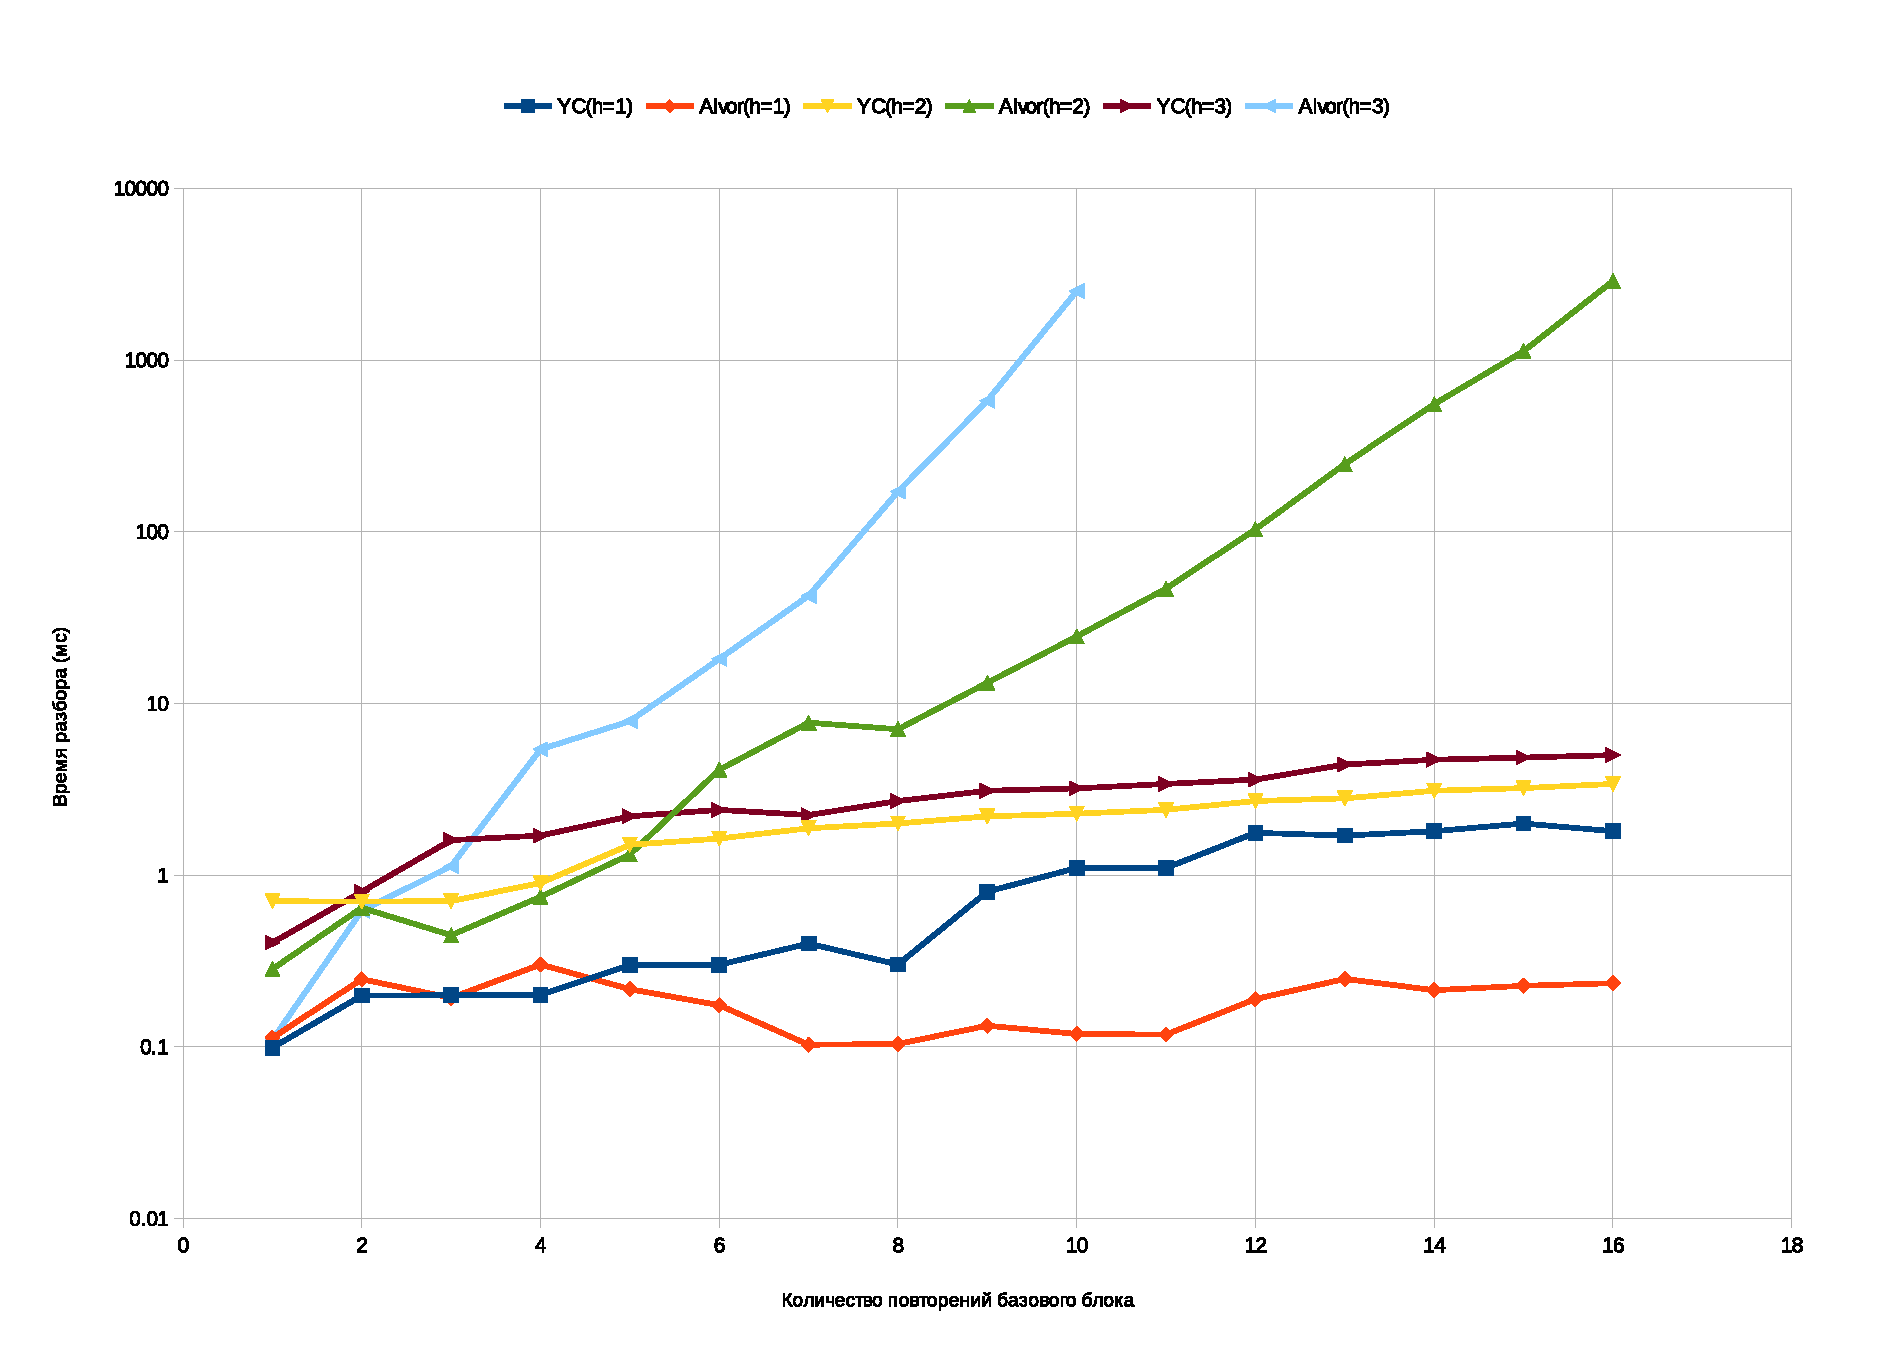
\includegraphics[width=0.95\textwidth]{pics/AlvorVsYC.eps}
 \caption{Сравнение производительности Alvor и синтаксического анализатора на базе YC.SEL.SDK}
 \label{fig:YCvsAlvor}
\end{figure}


\begin{table} [htbp]
  \centering
  \parbox{14cm}{\caption{Результаты сравнения производительности Alvor и синтаксического анализатора на базе YC.SEL.SDK}\label{tbl:YCvsAlvor}}
  \begin{tabular}{| r | c | c | c | c | c | c |}
  \hline                               
  \hline
  \textnumero & YC(h=1) & Alvor(h=1) & YC(h=2) & Alvor(h=2) & YC(h=3) & Alvor(h=3)\\
  \hline 
1 &  0.099 &  0.113 &  0.706 &  0.284   & 0.405 &  0.11     \\
2 &  0.199 &  0.248 &  0.702 &  0.646   & 0.801 &  0.622    \\
3 &  0.2   &  0.193 &  0.707 &  0.447   & 1.601 &  1.129    \\
4 &  0.201 &  0.302 &  0.901 &  0.748   & 1.701 &  5.403    \\
5 &  0.3   &  0.217 &  1.502 &  1.32    & 2.203 &  7.89     \\
6 &  0.301 &  0.175 &  1.635 &  4.114   & 2.402 &  18.187   \\
7 &  0.4   &  0.103 &  1.877 &  7.734   & 2.24  &  42.447   \\
8 &  0.302 &  0.104 &  2.002 &  7.076   & 2.704 &  171.529  \\
9 &  0.802 &  0.133 &  2.202 &  13.204  & 3.104 &  580.545  \\
10&  1.102 &  0.119 &  2.282 &  24.578  & 3.204 &  2521.318 \\
11&  1.102 &  0.118 &  2.404 &  46.662  & 3.403 &           \\
12&  1.766 &  0.19  &  2.704 &  103.417 & 3.605 &           \\
13&  1.701 &  0.249 &  2.803 &  248.107 & 4.408 &           \\
14&  1.803 &  0.214 &  3.103 &  554.314 & 4.706 &           \\
15&  2.001 &  0.227 &  3.217 &  1125.976& 4.843 &           \\
16&  1.803 &  0.235 &  3.403 &  2886.261& 5.006 &           \\
  \hline
  \hline

  \end{tabular}
\end{table}

В результате измерений выяснено, что производительность реализованного алгоритма синтаксического анализа лучше чем производительность аналогичного алгоритма, реализованного в инструменте Alvor на входных данных, содержащих большое количество ветвлений. При этом, Alvor не строит деревья разбора, в отличии от алгоритма, реализованного в данной работе.
